\documentclass{report}
\usepackage[T1]{fontenc} % Fontes T1
\usepackage[utf8]{inputenc} % Input UTF8
\usepackage[backend=biber, style=ieee]{biblatex} % para usar bibliografia
\usepackage{csquotes}
\usepackage[portuguese]{babel} %Usar língua portuguesa
\usepackage{blindtext} % Gerar texto automaticamente
\usepackage[printonlyused]{acronym}
\usepackage{hyperref} % para autoref
\usepackage{graphicx}
\usepackage{indentfirst}
\bibliography{bibliografia}

\begin{document}

%%
% Definições
%
\def\titulo{Sistemas de Armazenamento de Dados}
\def\data{14/11/2017}
\def\autores{Afonso Cardoso, Pedro Almeida}
\def\autorescontactos{(88964) afonsocardoso@ua.pt, (89205) pedro22@ua.pt}
\def\versao{VERSAO}
\def\departamento{Departamento de Electrónica, Telecomunicações e Informática}
\def\empresa{Universidade De Aveiro}
\def\logotipo{ua.pdf}
%

%%%%%% CAPA %%%%%%
%
\begin{titlepage}

\begin{center}
%
\vspace*{50mm}
%
{\Huge \titulo}\\ 
%
\vspace{10mm}
%
{\Large \empresa}\\
%
\vspace{10mm}
%
{\LARGE \autores}\\ 
%
\vspace{30mm}
%
\begin{figure}[h]
\center
\includegraphics{\logotipo}
\end{figure}
%
\vspace{30mm}
\end{center}
%
\begin{flushright}
\versao
\end{flushright}
\end{titlepage}

%%  Página de Título %%
\title{%
{\Huge\textbf{\titulo}}\\
{\Large \departamento\\ \empresa}
}
%
\author{%
    \autores \\
    \autorescontactos
}
%
\date{\data}
%
\maketitle

\pagenumbering{roman}

%%%%%% RESUMO %%%%%%
\begin{abstract}

	Os sistemas de armazenamento de dados provêm da necessidade do ser humano produzir e guardar informação para fins industriais a princípio, contudo a ambição do homem levou a que estes dispositivos evoluíssem de maneira tal a que hoje em dia sejam responsáveis pela manutenção de informação importante e essencial à continua evolução do mundo tecnológico e todo o que este engloba.
	Os dispositivos evoluíram ao longo da história, sendo protagonistas desta evolução variadas pessoas e empresas. Começaram por ter um formato simples e direto, adequado à necessidade da altura, e a partir de então adaptaram-se a diferentes situações e tecnologias, aumentado o seu armazenamento e mudando a sua estética. 
	Uma das vertentes da tecnologia, é que esta pode ter diferentes níveis de aceitação para diferentes produtos, influenciando assim o desenvolvimento dos mesmos. No caso dos dispositivos de armazenamento de dados, estes receberam um elevado nível de aceitação, levando assim ao seu elevado desenvolvimento, estando hoje em dia presentes na maior parte dos nossos produtos informáticos, sejam computadores, smartphones, câmaras e até mesmo relógios.
	Os dados são memorizados na forma de código binário, assim tem sido desde o primeiro dispositivo, e assim permaneceu até os dias de hoje. Os dispositivos aqui apresentados possuem algumas semelhanças e diferenças aquando do processo de armazenamento, porém estes são descritos e explicados, sendo possível assim estabelecer uma relação entre eles.

\end{abstract}

%%%%%% Agradecimentos %%%%%%
% Segundo glisc deveria aparecer após conclusão...
\renewcommand{\abstractname}{Agradecimentos}
\begin{abstract}
Eventuais agradecimentos.
Comentar bloco caso não existam agradecimentos a fazer.
\end{abstract}

\tableofcontents
\listoftables     % descomentar se necessário
\listoffigures    % descomentar se necessário


%%%%%%%%%%%%%%%%%%%%%%%%%%%%%%%
\clearpage
\pagenumbering{arabic}

%%%%%%%%%%%%%%%%%%%%%%%%%%%%%%%%
\chapter{Introdução}
\label{chap.introducao}
%Introduz o tema, apresenta a motivação e finalmente a estrutura.
	Com a evolução da tecnologia e o surgimento das primeiras invenções mecanizadas, surgiu a necessidade de guardar dados e informações importantes. Assim, como resposta a este problema, teve de ser criado algo com a capacidade de registar e guardar essa informação. O que foi criado foram dispositivos de armazenamento de dados, sendo o primeiro o \textit{Punched card} (Cartão perfurado), utilizado pela primeira vez em 1725. 
\vspace{1mm}
	
	Contudo, na atualidade, o armazenamento de dados não é utilizado apenas pelas industrias mas também para utilização pessoal. Todos sentem a necessidade de guardar algo, seja qual for a utilidade ou fim. "Dados são conhecimento, é um pedaço de história, um fragmento de algo ou um todo de uma vida"[1].
\vspace{1mm}
	
	Estes dispositivos de armazenamento têm vindo a sofrer um processo de evolução ininterrupto até aos dias de hoje. Tendo sempre como base as suas origens e como visão, o aumento da sua capacidade de armazenamento, o aumento da velocidade de acesso à informação guardada, assim como, a redução das dimensões físicas dos sistemas de armazenamento.
\vspace{1mm}
	
	Uma alteração que acontece na atualidade em novos computadores, é a substituição do muito usado e comum disco rígido pelo \ac{ssd}. Assim como este exemplo dado, houve muitas outras inovações que levaram a tecnologia anterior a entrar em desuso, como irá ser descrito com mais pormenor mais à frente.
\vspace{2mm}
%motivaçao	

	Estas evoluções e mudanças na área do armazenamento de dados foi, sem dúvida, o que despertou o interesse para a elaboração deste trabalho, pretendendo, assim, descobrir a origem e a história destes sistemas até aos dias de hoje.
\vspace{2mm}


Este documento está dividido em quatro capítulos.
Depois desta introdução, no \autoref{chap.metodologia} é apresentada a metodologia seguida.
	No \autoref{chap.evolucao} são apresentados todos os sistemas de armazenamento de dados até à atualidade, ordenados por ordem cronológica. 
	Finalmente, no \autoref{chap.conclusao} são apresentadas
as conclusões do trabalho.

\chapter{Metodologia}
\label{chap.metodologia}
Descreve os métodos utilizados para obtenção de resultados.

Neste esqueleto de relatório aproveitamos este capítulo para exemplificar
como se usam alguns elementos de {\LaTeX}.

\newpage

\chapter{Evolução de Sistemas de Armazenamento de Dados}
\label{chap.evolucao}
	\section{Cartão Perfurado}	
		
		O Cartão Perfurado(\textit{Punched Card} foi inventado por Joseph-Marie Jacquard em 1804 para o comando automático de teares depois de ter percebido que as mudanças de linhas coloridas e novelos  seguiam uma certa lógica. Deste modo, Jacquard inventou um processo de cartões perfurados que definiam padrões nas lançadeiras e assim o trabalho do tecelão seria trocado para algo "automático". 
		
		Os cartões perfurados contêm informações digitais representadas pela presença ou falta de furos em posições predefinidas. O método foi interessante para codificar as informações e do ano 1900 a 1950, foram o principal meio de entrada de dados, armazenamento de dados e processamento na computação institucional, tudo pela mão da \ac{ibm}. 
		
		Apesar de várias melhorias ao longo dos anos, com o desenvolver das tecnologias, os cartões perfurados não conseguiam suprir as necessidades e acabaram por ser substituídos.
		
		\begin{figure}[h]
		\centering
		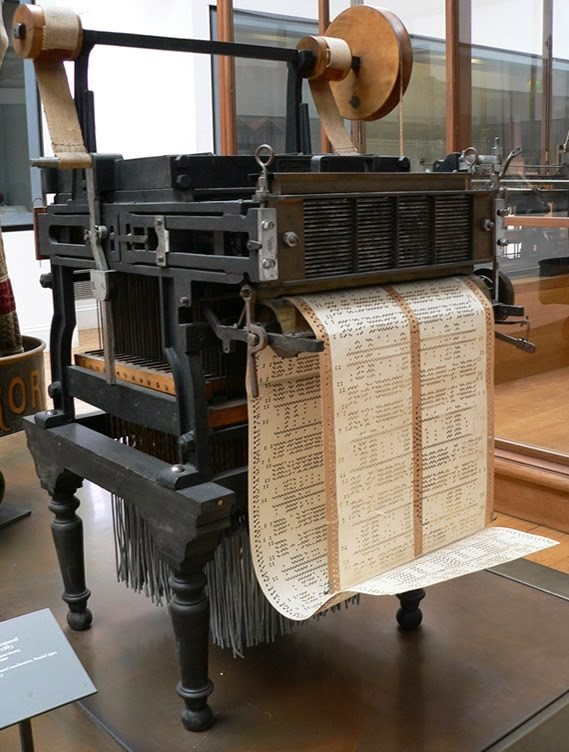
\includegraphics[width=3cm, height=4cm]{cartaoperfurado.jpg}
		\caption{Cartão Perfurado}
		\end{figure}
\newpage

		\section{Tubo de Williams}
		O Tubo de Williams é um tipo de memória para computadores criada por Sir Frederick Williams no ano de 1947 na Universidade Manchester tendo sido usado dois anos mais tarde na construção do computador Manchester Mark I.
	
	Este foi o primeiro dispositivo digital de memória de acesso aleatório e foi utilizado com sucesso em vários computadores antigos e possuía uma velocidade de 1,2 milésimos de segundo por instrução, o que na altura era algo bastante inovador.
	
	No seu processo de armazenamento de informação, um eletrão percorre sucessivas linhas na face do tubo, marcando com pontos ou traços de carga elétrica florescente na placa representando assim os uns e os zeros do código binário.
	
	Os primeiros computadores utilizavam este tipo de memória de tubos de raios catódicos (feixes de eletrões), díodo-condensador (mantém a corrente a circular apenas num sentido) e também as memórias de linha de retardo que consistiam num tubo de aproximadamente 150 cm de comprimento contendo mercúrio, com um cristal de quartzo em cada ponta onde os dados a armazenar passavam pelo mercúrio na forma de vibrações mecânicas e eram reconvertidos na outra ponta.
\vspace{10mm}

	\begin{figure}[h]
		\centering
		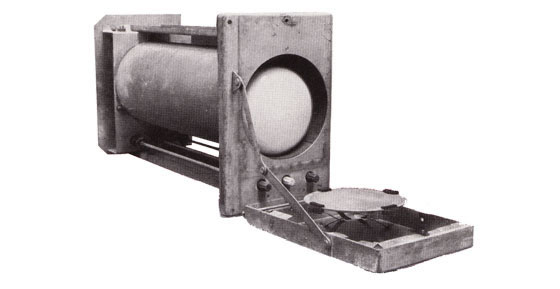
\includegraphics[width=5cm, height=3cm]{williamstube.jpg}
		\caption{Tube de Williams}
		\end{figure}	
\newpage

		
		\section{Tambor de Memória}
		 O tambor de memória, também conhecido como\textit{ Drum Memory} foi inventado por Gustav Tauschek em 1932 na Áustria e foi amplamente usado na década de 1950 e na década de 1960.
		 O tambor magnético é constituído por um cilindro de revolução metálico que roda em torno de um eixo vertical e o movimento é assegurado por um motor elétrico. Um conjunto de cabeças fixas assegura a gravação e a leitura da informação
		 
		 A capacidade de armazenamento do tambor de memória original tinha uma capacidade de cerca de 500,000 bits. Este sistema de armazenamento de dados foi especialmente importante pois, no início da década de 60 passaram a utilizar-se na construção de computadores com memórias não voláteis, isto é, não perde a informação guardada depois de desligar a fonte de energia. Estas memórias eram construídas com ferrites e marcam um grande avanço tecnológico na área do armazenamento de dados.
\vspace{30mm}	
	
	\begin{figure}[h]
		\centering
		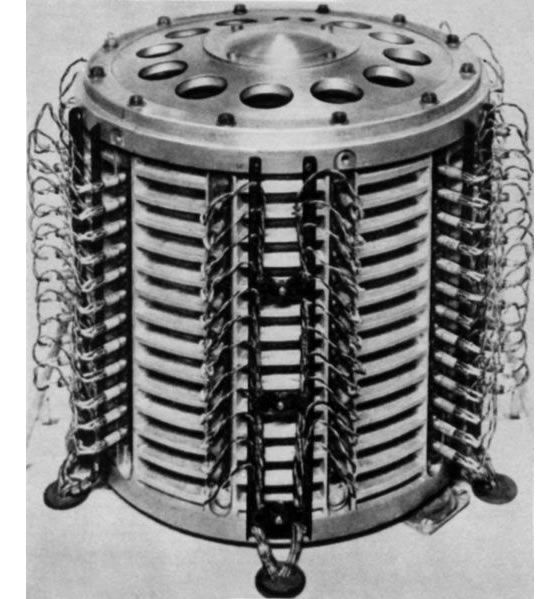
\includegraphics[width=4cm, height=6cm]{tambordememoria.jpg}
		\caption{Tambor de Memória}
		\end{figure}

\newpage

	\section{UNISERVO}

	A unidade de fita \textit{UNISERVO}  , introduzido a 1951, foi o principal dispositivo de I/O (os dados entram através de código ou programa para um hardware, assim como a sua saída ou retorno de dados) no computador \textit{UNISERVO I} . O seu lugar ficou garantido na história pois este dispositivo foi a primeira unidade de fita para um computador vendido comercialmente. 
\vspace{1mm}	
	
	O \textit{UNISERVO}  usava uma fita de metal, com 13 mm de largura, feita de uma liga níquel-bronze de fósforo (chamado Vicalloy) e tinha 1200 metros de comprimento, e sendo esta incrivelmente pesada.
\vspace{1mm}
	
	Os dados são guardados em 8 secções da fita, onde 6 são para os valores dos dados (1 ou 0), 1 para a verificação de erros e 1 que regista o tempo, tudo isto à densidade de 128 bits por 2,54 cm. A fita pode ser movida a 254 cm por segundo, oferecendo uma taxa de transferência nominal de 12,800 caracteres por segundo. Os blocos onde os dados são guardados possuem o tamanho fixo de 60 palavras de 12 caracteres cada.
\vspace{1mm}
	
	O \textit{UNISERVO}  ao longo dos anos foi sofrendo várias melhorias e atualizações para ser capaz de ler dados através de outras fitas metálicas.

\begin{figure}[h]
		\centering
		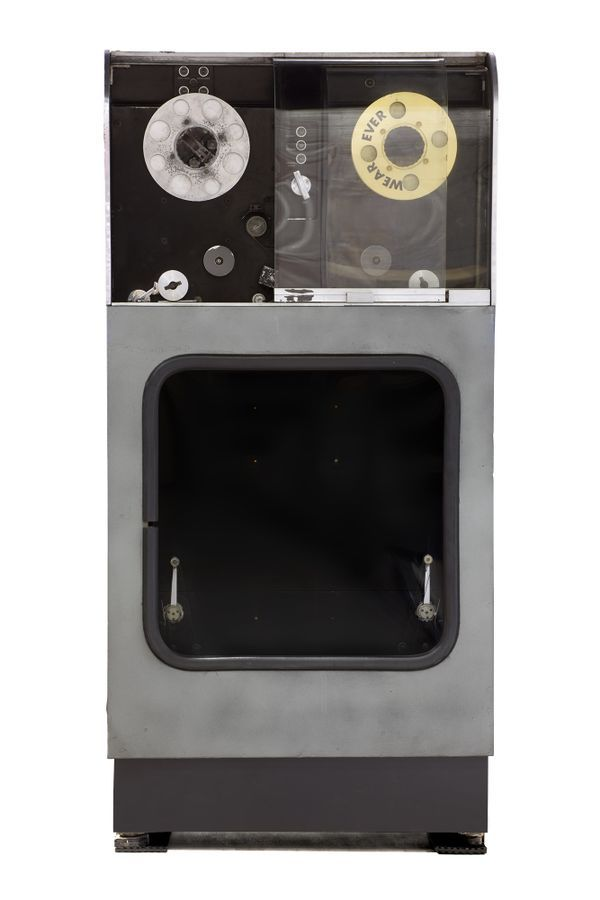
\includegraphics[width=4.7cm, height=7cm]{uniservo.jpg}
		\caption{O UNISERVO}
		\end{figure}
	
\newpage
		\section{IBM 350 Disk Storage Unit}
		
		Em 1956, a \ac{ibm} lançou no mercado o IBM 305 \ac{ramac}, o primeiro computador produzido em série para empresas, visto que até aqui, os computadores eram exclusivos para aplicações militares. Assim, o \ac{ramac}, foi projetado para executar aplicativos de contabilidade e controlo de transações comercias, tais como processamento de pedidos, controlo de inventário e folhas de pagamentos.
\vspace{1mm}

		A novidade que o computador 305 \ac{ramac}, que era equipado com 350 Disk Storage Unit, não era a sua capacidade de processamento, mas na utilização de um novo equipamento periférico para a entrada e saída de dados, o qual permitia a gravação e leitura de dados de forma muito mais rápida comparada com os outros sistemas de armazenamento usados até então.
\vspace{1mm}
		
		A novidade que o computador 305 \ac{ramac}, que era equipado com 350 Disk Storage Unit, não era a sua capacidade de processamento, mas na utilização de um novo equipamento periférico para a entrada e saída de dados, o qual permitia a gravação e leitura de dados de forma muito mais rápida comparada com os outros sistemas de armazenamento usados até então. Ao possibilitar que a informação fosse gravada, lida e alterada em poucos segundos e, principalmente, pudesse ser feito o acesso de forma aleatória, eliminou a necessidade de se classificar os dados em sequência antes do seu processamento, o que até então era um requisito imposto pelos equipamentos de fita magnética ou cartões perfurados, que eram os meios disponíveis para se armazenar dados até ao momento.
\vspace{1mm}

		 O \ac{ramac} pôs fim da era dos cartões perfurados e introduziu uma nova. As corporações passaram a utilizar computadores para realizar negócios, fazendo uso do processamento de transações online e armazenamento de grandes volumes de dados em discos magnéticos. Realçando a importância da tecnologia introduzida no \ac{ramac} e como influenciou por completo no modo de armazenar e processar a informação, ainda na atualidade, apesar de muitos melhoramentos, a tecnologia para produzir discos magnéticos é a mesma. Contudo, 1961 foi o último ano de produção.

	\begin{figure} [h]
		\centering
		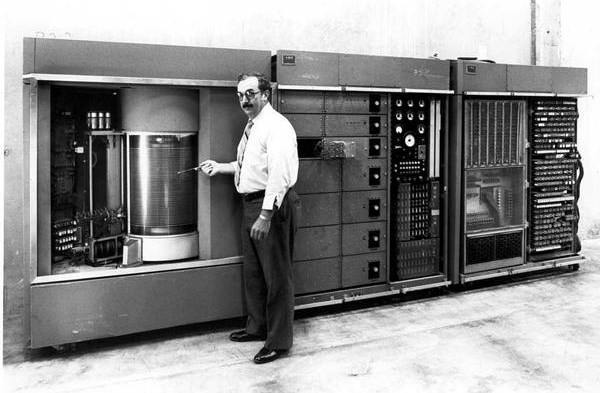
\includegraphics[width=6cm, height=4cm]	{RAMAC.jpg}
		\caption{IBM 350 RAMAC}
	\end{figure}
	
\newpage
		
		\section{Cassete}	
	A cassete ou \textit{compact cassette}  é um padrão de fita magnética para gravação de áudio lançada oficialmente em 1963, invenção da empresa holandesa \textit{Philips}, possuindo um armazenamento de 660 \ac{kb} por cada lado da cassete. Possui também a abreviação de: "K7".
\vspace{1mm}
	
	A cassete era constituída basicamente por 2 carretos, a fita magnética e todo o mecanismo de movimento da fita alojados numa caixa plástica. Esta fita é coberta por uma substância à base de ferro, estando presente nesta milhões de ímanes pequenos que formam um campo magnético. Ao gravar dados, as partículas ordenam-se de modo a ser possível a gravação.
\vspace{1mm}

	Isto facilitava o manuseamento e a utilização permitindo que a fita fosse colocada ou retirada em qualquer ponto da reprodução ou gravação sem a necessidade de ser rebobinada como as fitas de rolo. 
\vspace{1mm}
	
	Com um tamanho de 10 por 7 cm, a caixa plástica permitia uma enorme economia de espaço e uma excelente utilização face às fitas tradicionais.
\vspace{1mm}

	No início, era possível gravar apenas 30 minutos em cada lado da fita, perfazendo assim uma hora de gravação. Se usasse mais tempo, a qualidade do som diminuía. Ao longo do tempo, foram acrescentados recursos tecnológicos e as fitas passaram a armazenar conteúdo até 45, 60, 90 e até 120 minutos. A invenção representava uma revolução na época, pois ampliava as possibilidades de reproduzir música, e finalmente, ao surgir os famosos \textit{Walkman}  , fez crescer o aumento de utentes da cassete aumentar drasticamente.
\vspace{1mm}

	Inicialmente a expectativa era de colocar dados neste suporte, mas o seu preço levou a que fosse posta de parte, favorecendo assim o surgimento disquete.
	
	\begin{figure} [h]
		\centering
		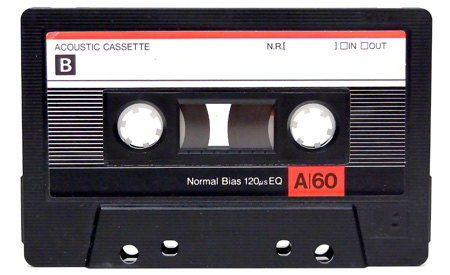
\includegraphics[width=8.19cm, height=5cm]{cassete.jpg}
		\caption{Cassete}
	\end{figure}		
		
\newpage

		\section{Disquete}
		A Disquete, também conhecido como \ac{fdd}, foi desenvolvida no final da década de 60 mas só ficou disponível comercialmente em 1971 com um tamanho inicial de 8 polegadas e com uma capacidade de armazenamento de dados de 80 KB. Muito resumidamente, uma disquete é um disco protegido por uma capa para evitar que se danifique. 
\vspace{1mm}

		Disquetes podem ser lidas e gravadas por um leitor de disquete, chamado também de \ac{fdd}. As disquetes possuem a mesma estrutura de um disco rígido sendo todos periféricos de entrada e saída mas podendo estas ser removíveis e serem compostas apenas por um único disco magnético.
\vspace{1mm}
		
		 Devido à fácil utilização, a disquete foi, por mais de duas décadas, o principal sistema de armazenamento de dados mais utilizado. A maioria dos ambientes computacionais antes de 1990 não possuíam redes, e assim, as disquetes eram o principal sistema de transferência de dados entre os computadores.
\vspace{1mm}
		
		Contudo, vários motivos fizeram com que, com o passar dos anos, as disquetes acabassem em desuso. O principal foi a sua escassa capacidade de armazenamento em comparação com outras tecnologias mais avançadas (embora já tenha sido considerado um dispositivo com grande capacidade de armazenamento) que oferecem como, por exemplo, \ac{cd-rom} que irá ser analisado mais tarde. Outra causa para o desuso das disquetes, era a facilidade com que se danificavam fosse por estarem perto de um campo magnético exterior ou por acumulação de sujidade.
\vspace{1mm}
	
		Disquetes podem ser lidas e gravadas por um leitor de disquete, chamado também de \ac{fdd}. As disquetes possuem a mesma estrutura de um disco rígido sendo todos periféricos de entrada e saída mas podendo estas ser removíveis e serem compostas apenas por um único disco magnético.
\vspace{1mm}
		
	\begin{table}[h]
		\centering
		\caption{Evolução da Disquete}
		\vspace{2mm}
		\label{Tabela de Disquete}
		\begin{tabular}{|l|l|l|}
		\hline
		\textbf{Tipo de Disco} & \textbf{Ano} & \textbf{Capacidade} \\ \hline
		8 pol            & 1971 & 80 kB   \\ \hline
		8 pol            & 1973 & 256 kB  \\ \hline
		8 pol            & 1974 & 800 kB  \\ \hline
		8 pol dual-sided & 1975 & 1 MB    \\ \hline
		1.25 pol         & 1976 & 160 kB  \\ \hline
		1.25 pol         & 1978 & 360 kB  \\ \hline
		1.25 pol         & 1980 & 720 kB  \\ \hline
		1.25 pol         & 1984 & 1.2 MB  \\ \hline
		3 pol            & 1984 & 320 kB  \\ \hline
		1.5 pol          & 1984 & 720 kB  \\ \hline
		1.5 pol          & 1987 & 1.44 MB \\ \hline
		1.5 pol          & 1991 & 2.88 MB \\ \hline
		1.5 pol          & 1993 & 5.76 MB \\ \hline
		
		\end{tabular}
		\end{table}		
 
	Analisando a tabela, pode concluir-se que, ao longo dos anos, a dimensão física tem tendência a diminuir, inversamente à capacidade de armazenamento de dados que vai aumentando. A disquete passou também a ler dados em vez de só os gravar. 

	\textbf{Facto:}	
		\begin{itemize}
		 	\item As disquetes foram os primeiros transmissores de vírus de computador. 
	 	\end{itemize}
	
	
	\begin{figure} [h]
		\centering
		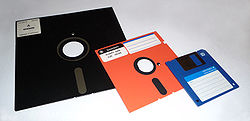
\includegraphics[scale=1]{disquete.jpg}
		\caption{Disquete}
	\end{figure}
	
\newpage		
		
		\section{IBM 3380}	
	O IBM 3380 \ac{dasd} foi anunciado em Junho de 1980 pela IBM. Foi desenvolvido pela Universidade de Auckland e foi o primeiro dispositivo de armazenamento a atingir o território do Gigabyte, ficando ,assim, na história por esse mesmo feito.
		
	O IBM 3380 \textit{Direct Access Storage Device}  foi anunciado em Junho de 1980 pela IBM. Foi desenvolvido pela Universidade de Auckland e foi o primeiro dispositivo de armazenamento a atingir o território do Gigabyte, ficando ,assim, na história por esse mesmo feito.
\vspace{1mm}
	
	Os vários modelos da série 3380 ((A4, A4F, AA4, AAF, B4 e BF4), eram uma apenas uma solução de armazenamento de dados, não eram o próprio computador. Todos esses modelos usavam duas \textit{hard drives} com cerca de 1.26 \ac{gb} cada, perfazendo, assim, um total de 2.52 GB. Tinha uma taxa de 3 \ac{mb} por segundo de transferência de dados. O tempo médio de acesso era de 16 ms (milissegundos). O seu peso era de aproximadamente 29 kg. 
\vspace{1mm}

	
	Apesar dos vários modelos da série 3380 terem todas características semelhantes, foram sempre recebendo melhoramentos. Comparando o primeiro modelo com o último, foi possível reduzir o consumo de energia em 70\% e a produção de calor em 75\%. Estes avanços, fizeram com que o \ac{ibm} 3380 se tornasse muito mais fiável e eficiente.
\vspace{1mm}

	O preço de adquirição deste equipamento no momento em que foi introduzido no mercado variou de 81,000 dólares a 142,200 dólares, dependendo do modelo.
\vspace{1mm}

	\begin{figure} [h]
		\centering
		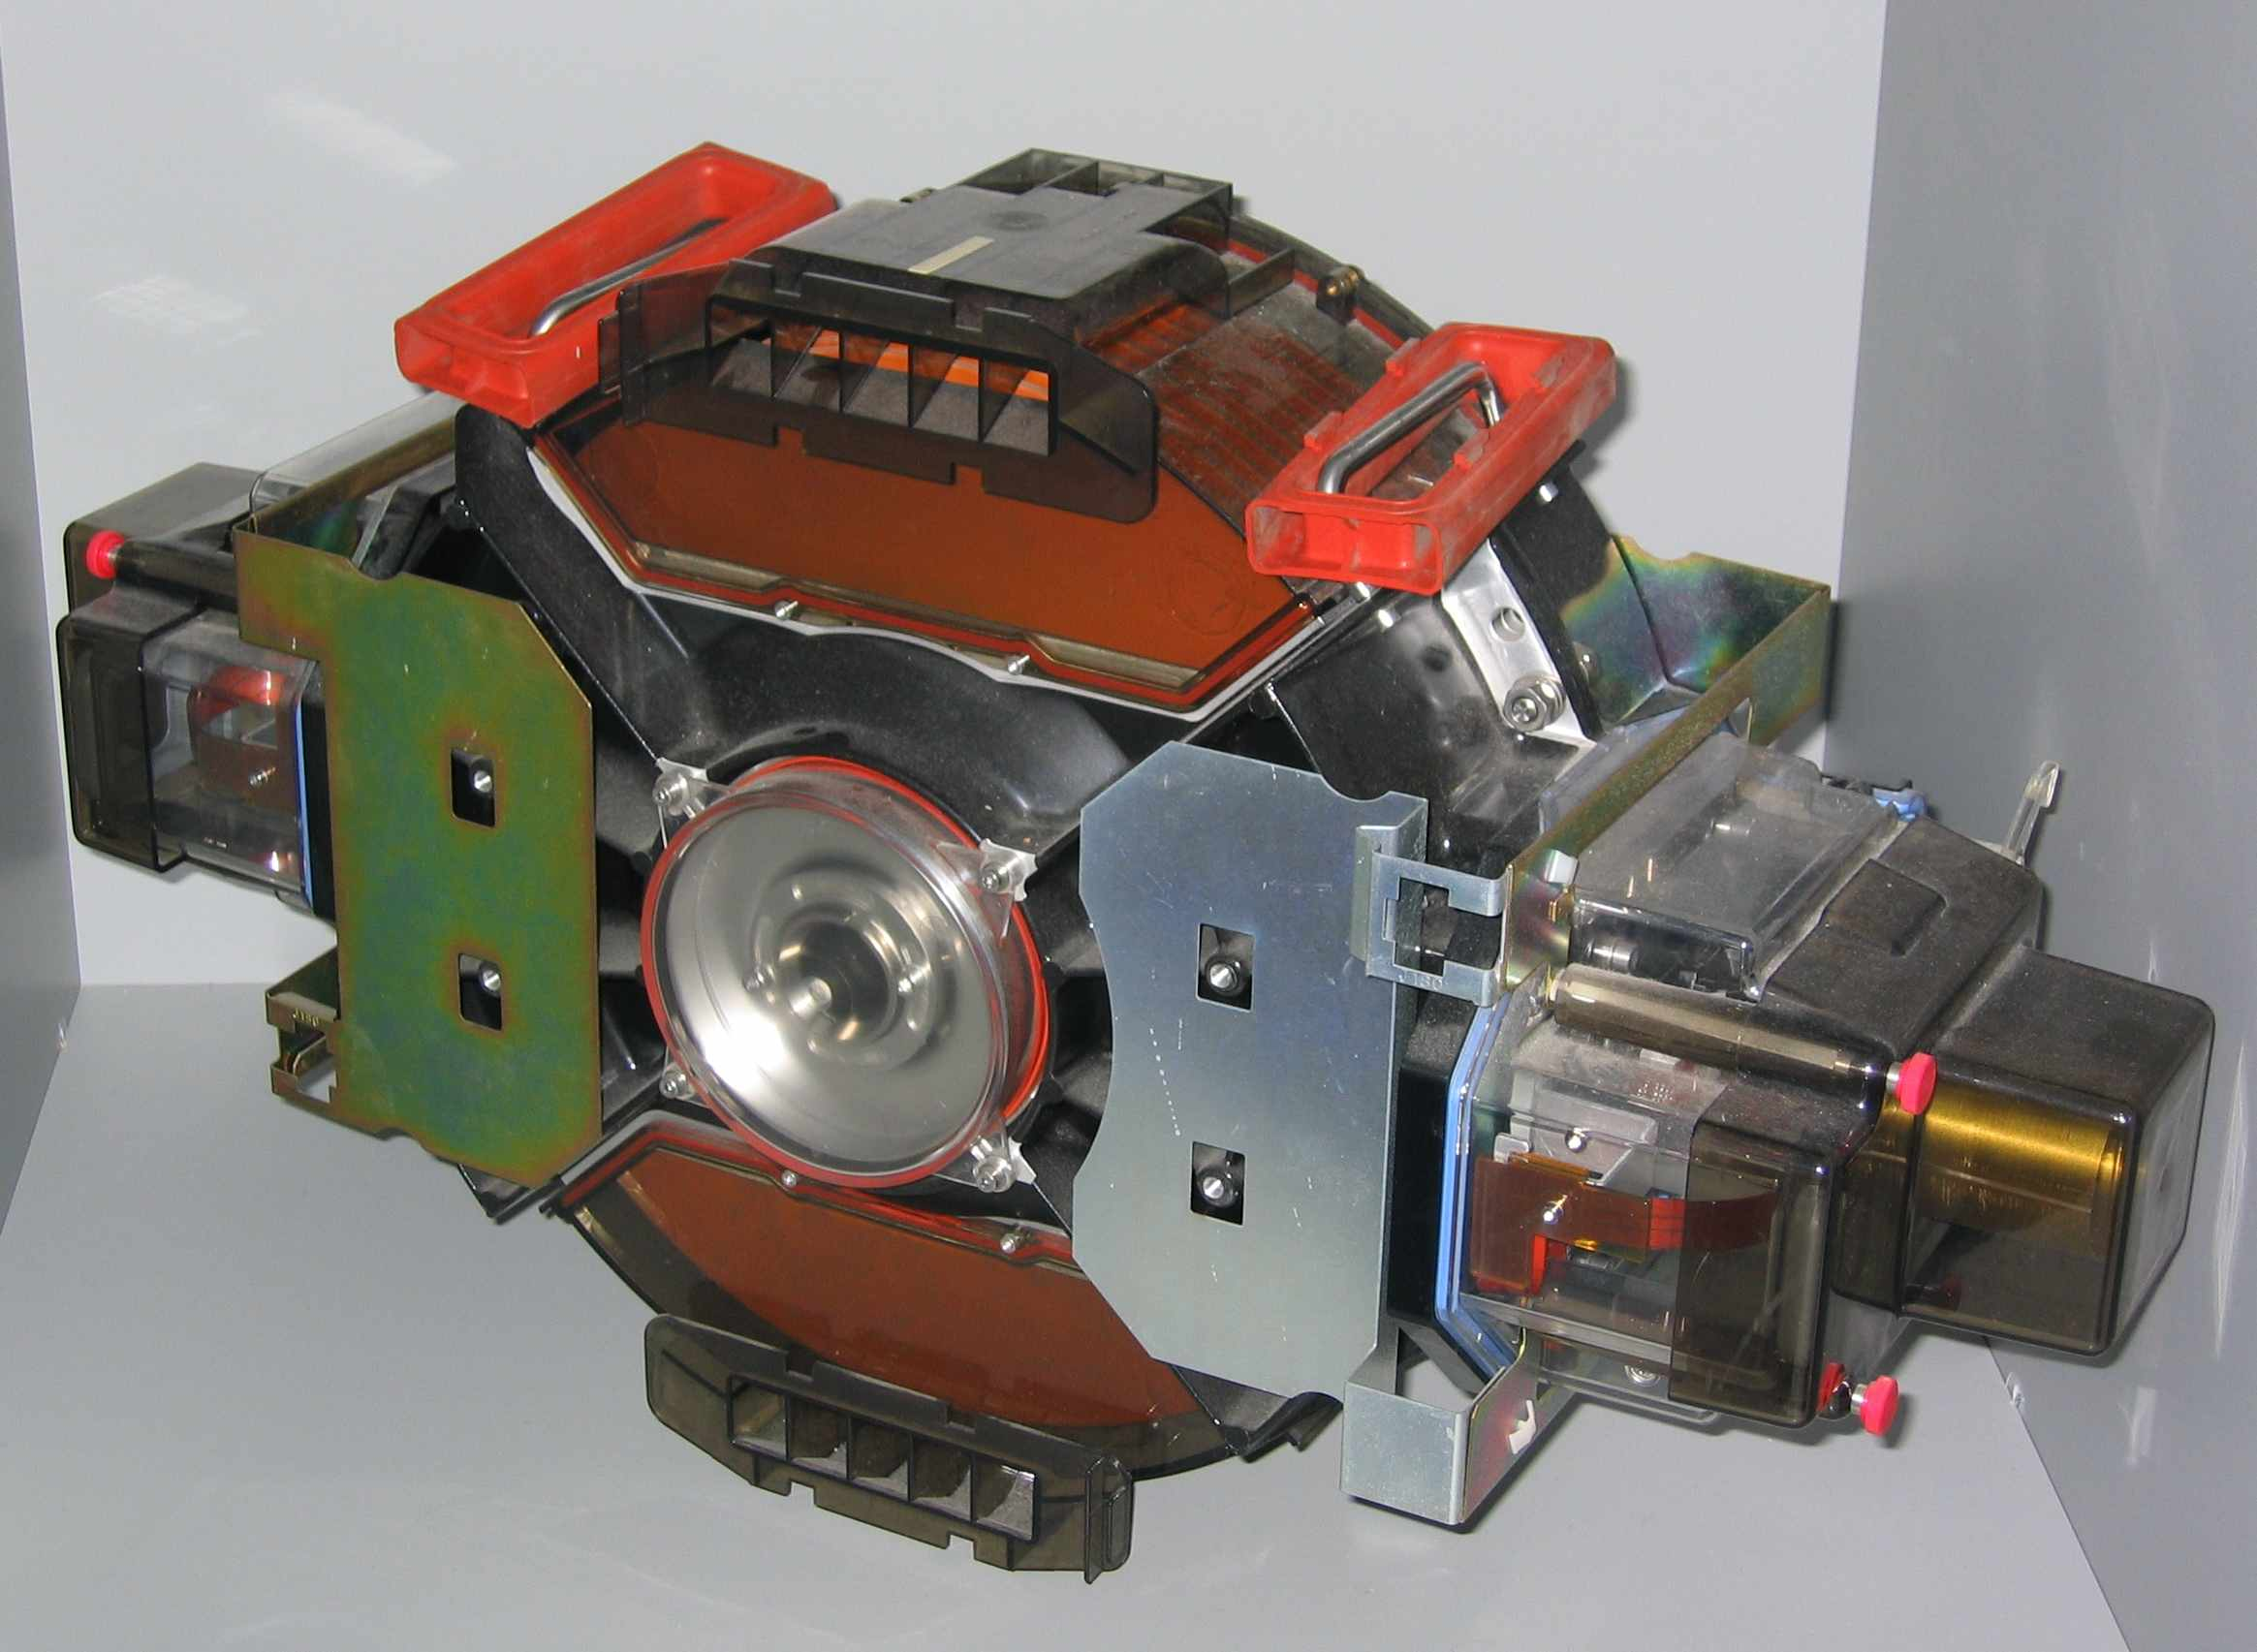
\includegraphics[scale=0.07]{ibm3380.jpg}
		\caption{Hard Drive Assembly (HDA)}
	\end{figure}

\newpage
		
		\section{ST-506}

	O ST-506 foi o primeiro disco rígido de 5.25 polegadas. Apresentado em 1980 pela então denominada \textit{Shugart Technology} (hoje \textit{Seagate Technology}), tinha uma capacidade de 5 \ac{mb} após formatação. 
\vspace{1mm}

	O ST-412 um modelo semelhante, mas muito mais caro, tinha um espaço de armazenamento de 10 \ac{mb} e foi lançado em fins de 1981. Ambos usavam codificação \ac{mfm} (um esquema de coficação em linha para codifcar informação na maioria dos modelos da disquete).
\vspace{1mm}
	
	Uma versão posterior do ST-412 usava RLL (uma técnica de codificação em linha que foi usada para enviar dados arbitrários por um canal de comunicações com largura de banda limitada) para um incremento de 50\% na capacidade e taxa de transferência.
\vspace{1mm}
	
	Esta foi a primeira drive com esta dimensão e foi quem deu origem aos atuais discos rígidos que utilozamos nos dias de hoje.
\vspace{1mm}

	O ST-506 estava presente na interface de um computador usando um controlador de disco. A interface do ST-506 era derivada da interface SA1000 da \textit{Shugart Associates}  a qual por sua vez era baseada na interface da unidade de disquetes tornando assim a fabricação de controladores de disco relativamente fácil.
\vspace{1mm}

	\begin{figure} [h]
		\centering
		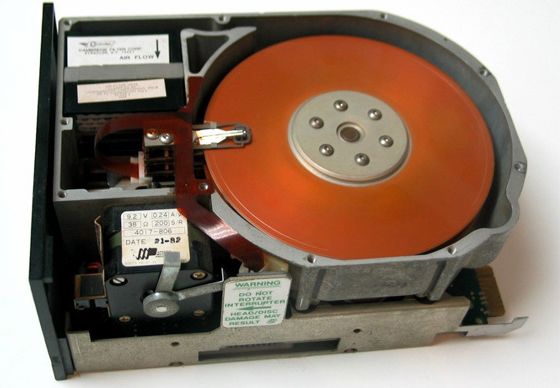
\includegraphics[scale=0.3]{st-506.jpg}
		\caption{O ST-506}
	\end{figure}		
\newpage

		\section{Digital Audio Tape}
	A \ac{dat} é um cassete de gravação digital apresentado pela Sony em 1987.	
	Funcionava com uma fita magnética de 4mm para fazer a gravação de dados. As fitas do \ac{dat} tinham entre 15 a 180 minutos de duração. Uma dita com 120 minutos tinha 60 metros de comprimento.
	
	A \ac{dat} nunca foi "adotada" em larga escala pelos consumidores. Isto aconteceu devido aos elevados custos mas viu uso em gravação professional.
	Sem grande sucesso, em 2005, a \textit{Sony} descontinuou a produção da \textit{Digital Audio Tape}.
	 
	
	\begin{figure} [h]
		\centering
		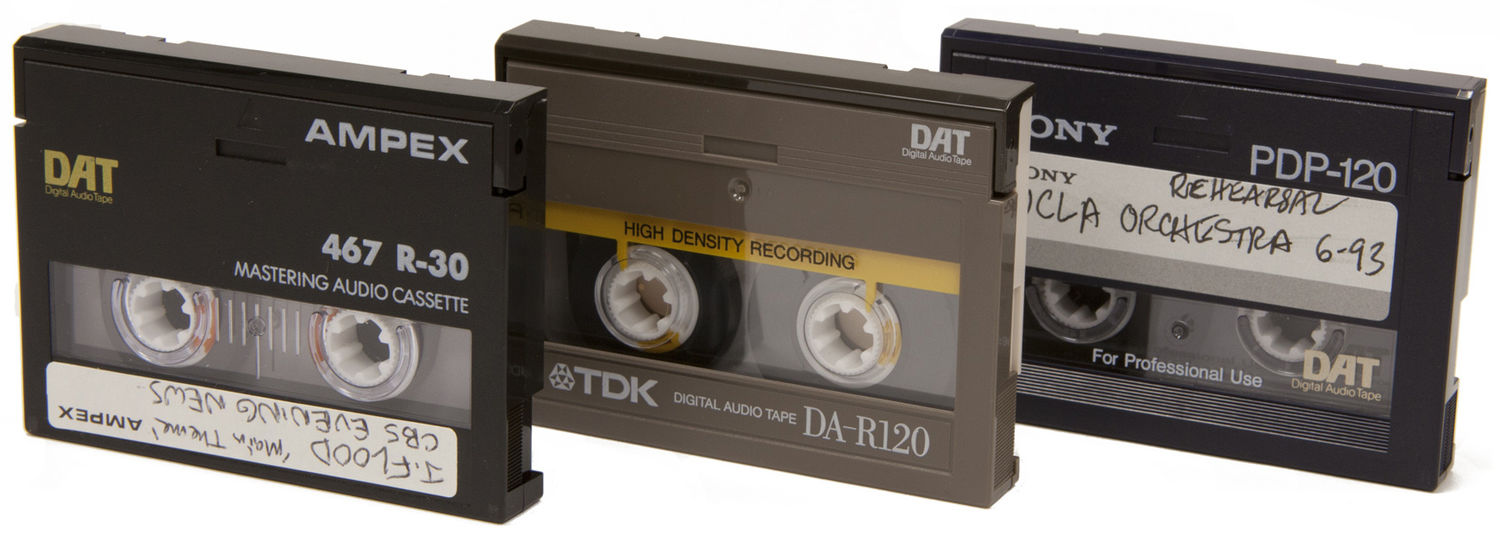
\includegraphics[scale=0.3]{dat.jpg}
		\caption{Digital Audio Tape}
	\end{figure}

\newpage
	

		\section{CD-R}
	
	Um \ac{cd-r} é um disco fino (1.2 mm) de poli-carbonato usado principalmente para gravar músicas ou dados, que surgiu no de 1990 com um armazenamento de 700 \ac{mb}. Mas em vez do alumínio usado nos CDs comuns para guardar os dados, o \ac{cd-r} usa uma camada especial de corante para permitir a gravação de dados num drive comum de \ac{cd-r}.
\vspace{1mm}

	Este suporte marcou a história pela sua ampla utilização e ainda atualmente consegue manter a sua presença tanto ao nível da gravação de música como de dados. Nem o ZIP Drive nem o JAZ Drive conseguiram destronar este suporte, o que fez dele um marco histórico no mundo dos dispositivos de armazenamento de dados.
\vspace{1mm}

	A superfície do \ac{cd} contém uma longa pista espiral de dados. Ao longo da pista, existem zonas lisas reflexivas e solavancos não reflexivos. A área lisa reflexiva representa o número binário 1, enquanto que o solavanco representa o número binário 0. O leitor de \ac{cd} emite um laser na superfície do \ac{cd} assim detetando ambas as áreas consoante a quantidade de luz que é refletida. Por fim o leitor converte as reflexões em 1's e 0's para ser feita a leitura dos seus dados. O \ac{cd-r} possui uma camada à mais que o laser poderá modificar, gravando assim dados.
\vspace{1mm}

	\begin{figure} [h]
		\centering
		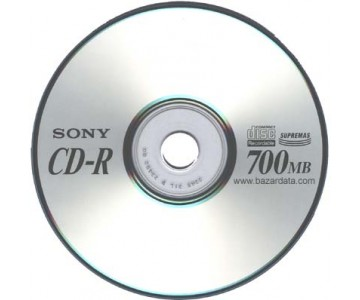
\includegraphics[scale=0.4]{cd-r.jpg}
		\caption{Um CD-R}
	\end{figure}

\newpage

		\section{MiniDisc Data}
		O 	\textit{MiniDisc Data}, também conhecido como \textit{MD Data} ou apenas \ac{md}, e como o nome indica, é, basicamente, um disco com capacidade de armazenamento de informação e normalmente privilegia o áudio. Foi anunciado pela Sony em 1991 mas apenas introduzida no mercado em 1992. 
Tinha uma capacidade de 140 \ac{mb} armazenamento.

	Contudo, o \ac{md}, à semelhança do Digital Audio Tape, nunca teve grande sucesso por várias razões:
	\begin{itemize} 
		\item era necessário estar em modo "play", logo não funcionava em computadores. O seu uso era predominante em câmeras digitais; 
		\item era muito caro;
		\item era considerado lento;
	\end{itemize} 
	
	Para contrariar o insucesso, a \textit{Sony} lançou, em 1997 o \textit{MD Data2}, que tinha mais capacidade de armazenamento, cerca de 650 \ac{mb}. Contudo, este formato só funcionava em outros dispositivos \textit{Sony}.
	Em 2013 foram vendidos os últimos exemplares.	

\begin{figure} [h]
	\centering
	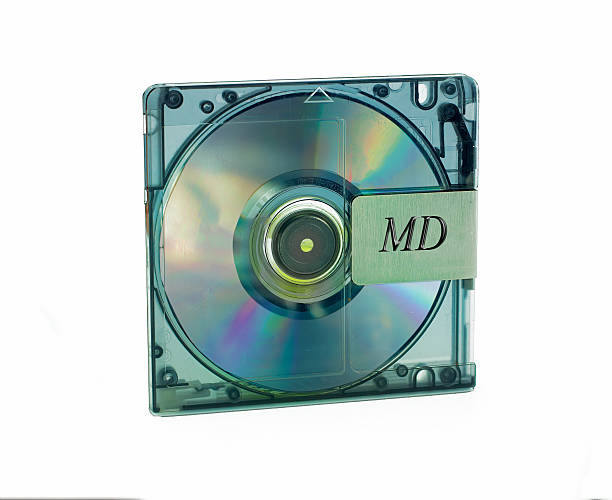
\includegraphics[scale=0.4]{MD_data.jpg}
	\caption{MiniDisc Data}
\end{figure}

\newpage	
			
		\section{ZIP}
	
	O ZIP Drive é um sistema de disco removível de média capacidade, introduzido pela \textit{Iomega} em 1994.
\vspace{1mm}

	O ZIP Drive foi baseado no sistema \textit{Bernoulli Box} da própria \textit{Iomega}; em ambos os sistemas, um conjunto de cabeças de leitura/escrita montado em atuadores lineares que flutuam em cima de uma disquete girando rapidamente, estando todas estas componentes dentro de um cartucho robusto. O ZIP Drive usa estruturas menores com aproximadamente o tamanho de uma disquete de 3,5 polegadas, em vez dos discos compactos como os suportes multimédia Bernoulli.
\vspace{1mm}

	Da junção de todas estas partes resultou um disco que possui toda a conveniência da disquete de 3,5 polegadas, mas armazena muito mais dados, com um maior desempenho que a \textit{floppy drive}, contudo não era diretamente competitivo com discos rígidos.
\vspace{1mm}
	
	O ZIP Drive original teve uma taxa de transferência de dados de cerca de 1 MB/s e um tempo de pesquisa de 28 milissegundos em média, comparado aos 500 kbit/s de taxa de transferência de uma disquete de 1.44 \ac{mb} e várias centenas de milissegundo de tempo de pesquisa.
\vspace{1mm}

	Este dispositivo ficou na história por ser uma solução de armazenamento escolhida pelas empresas e designers onde tinham uma drive rápida que era regravável e muito robusta. Aliada a isto estava o seu preço, muito mais em conta, face às alternativas.
\vspace{1mm}
	
	\begin{figure} [h]
		\centering
		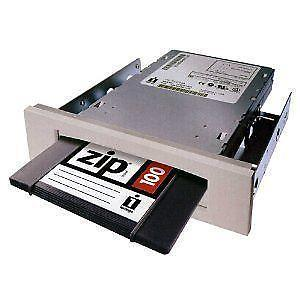
\includegraphics[scale=0.5]{zipdrive.jpg}
		\caption{Uma ZIP Drive e seu leitor}
	\end{figure}
	
\newpage

	\section{Seagate Barracuda}

	Seagate Barracuda é uma série do disco rígido, a maioria dos quais operam a uma velocidade de rotação de 7200 rpm (rotações por minuto). Eles são produzidos pela \textit{Seagate Technology}. Embora inicialmente fossem comercializados como unidades de alto desempenho com interfaces SCSI (a tecnologia que permite ao usuário conectar uma larga gama de periféricos, tais como discos rígidos) e capacidades elevadas para o seu tempo, uma vez que apareceram em 2001, tornaram-se no principal produto de mercado de massa da \textit{Seagate}. Com isto a indústria dos discos rígidos começou a colocar estas unidades nas unidades de \textit{desktop}.
\vspace{1mm}

	Esta foi a primeira unidade com 7200 rpm tornando-se num \textit{standard} para a indústria dos discos rígidos e dos nosso computadores e isso marcou a história do armazenamento.
\vspace{1mm}
	
	Os dados são gravados na forma binária de 0 e 1. Estes são gravados em diferentes bandejas. Estas bandejas são feita de uma liga de alumínio não-magnética, vidro ou cerâmica e são revestidos com uma fina camada de material magnético. Finalmente, estas são separadas em pilhas e setores, onde as pilhas são circunferências concêntricas e os setores em fatias de forma circular no top das pilhas.
\vspace{1mm}
	
	O disco rígido guarda informação na forma de campos magnéticos. Os dados são guardados digitalmente na forma de pequenas zonas magnetizadas no prato onde cada zona representa um bit. Para escrever no disco, um campo magnético é colocado num pequeno campo numa das duas polaridades: Norte-Sul e Sul-Norte. A orientação determina o número binário a introduzir. Se a orientação for "N-S" representa o "1", caso seja "S-N" representa o "0". Esta polaridade é analisada por controladores integrados no disco rígido.
\vspace{1mm}

	\begin{figure} [h]
		\centering
		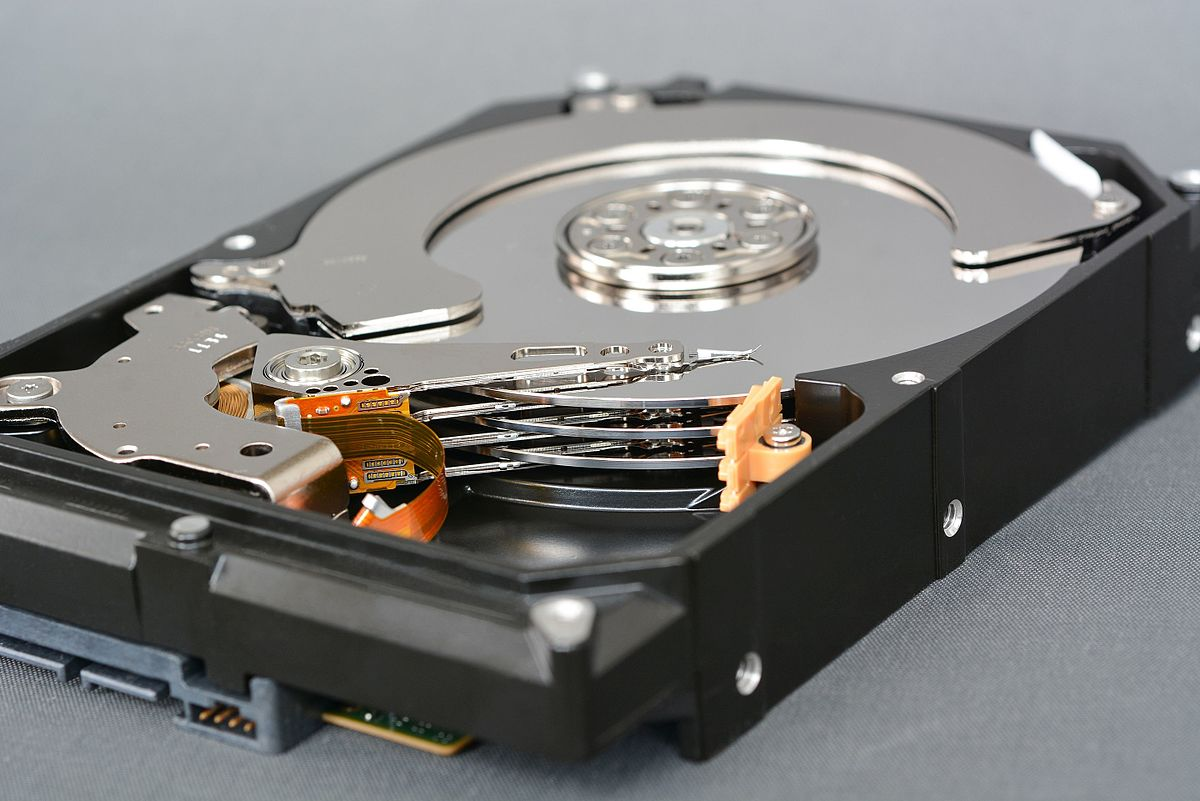
\includegraphics[scale=0.7]{barracuda.jpg}
		\caption{Seagate Barracuda}
	\end{figure}
	
\newpage
	
		\section{IBM 170 Microdrive}
	
	O \textit{Microdrive} (MD) é um disco rígido de 1 polegada concebido para caber num \textit{Slot Tipo II CompactFlash}.
	Este sistema de armazenamento de dados teve bastante adesão por ser barato, com bastante oferta e grande capacidade de armazenamento. 
	
	\begin{table}[h]
		\centering
		\caption{Modelos Microdrive} 
		\vspace{2mm}
		\label{Tabela de Microdive}
		\begin{tabular}{|l|l|}
		\hline
		\textbf{Ano} & \textbf{Armazenamento} \\ \hline
			1999 & 170  MB \\ \hline
			2000 & 512  MB \\ \hline
			2003 & 2  GB \\ \hline
			2004 & 2.5/5  GB  \\ \hline
			2005 & 6  GB  \\ \hline
			2006 & 8  GB  \\ \hline
			\end{tabular}
		\end{table}
	
	\begin{figure} [h]
		\centering
		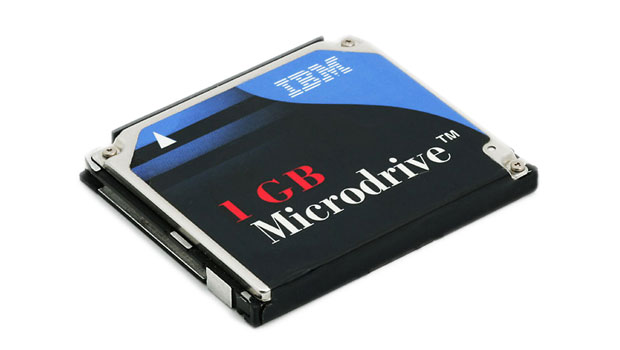
\includegraphics[scale=0.3]{microdrive.jpg}
		\caption{Microdrive}
	\end{figure}

\newpage
		
		\section{IBM DiskOnKey}	
		
		Em 2000, a \textit{M-Systems} e a \ac{ibm} apresentaram a \textit{IBM DiskOnKey}, também conhecida como \textit{USB drive}. A primeira unidade de armazenamento portátil que cabe num bolso e foi também a primeira unidade de armazenamento \textit{flash}  (armazenamento explicado mais à frente aquando dos cartões SD) comercializada.
\vspace{3mm}		
		 
	Com um tamanho de um polegar e com uma capacidade de armazenamento de 8 MB, as \textit{USB drive} revolucionaram as transferências de dados entre computadores. Era muito mais simples e rápido do que todos os métodos anteriores e não precisava de nenhum \textit{software} especial, apenas uma ligação USB, e foi, por isso mesmo, responsável por pôr fim à utilização das disquetes. As PEN's foram um sucesso imediato, apesar de o seu preço inicial não ser nada acessível.
\vspace{3mm}
	
	Os componentes internos de uma PEN estão tipicamente protegidos por um invólucro de plástico ou metal, o que o torna resistente para ser transportado num bolso. Assim, apenas o conector USB fica exposto, que muitas vezes é retrátil ou protegido por uma capa, o que torna o \textit{USB drive} bastante fiável.

\vspace{10mm}

	\begin{figure} [h]
		\centering
		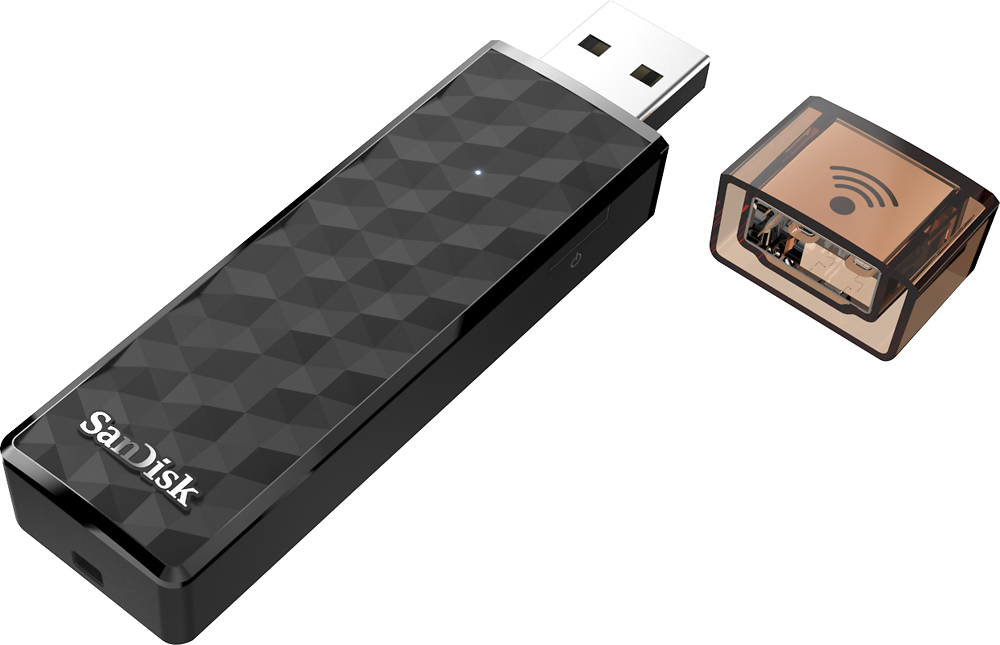
\includegraphics[scale=0.2]{pen.jpg}
		\caption{Wireless Pen Drive}
	\end{figure}

\newpage
	Na memória \textit{flash} a célula é composta por duas partes principais: o \textit{control gate} (também chamado de controlador) e o \textit{floating gate}. O controlador é a parte mais externa, que realiza a comunicação da memória com o computador e é responsável por ativar a célula. Os dados em si ficam armazenados no \textit{floating gate}, que por sua vez é isolado por duas camadas de óxido de silício dotadas de carga negativa.
	
	Para armazenar dados, uma carga elétrica é aplicada ao controlador. A tensão "empurra" alguns eletrões para o \textit{floating gate}, onde estes permanecem por causa das camadas de óxido. Quando a capacidade de carga ultrapassa os 50\%, é traduzido num "1", ao acontecer o contrário é traduzido "0". Enquanto uma nova carga não é aplicada, o conteúdo do \textit{floating gate} permanece inalterado, fazendo com que os dados possam ser lidos inúmeras vezes.
\vspace{1mm}

	\begin{figure} [h]
		\centering
		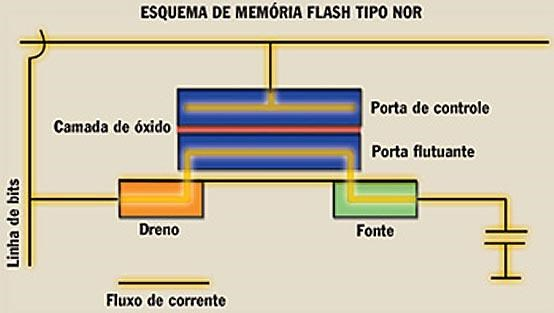
\includegraphics[scale=0.4]{flash.jpg}
		\caption{Processo de Memória Flash}
	\end{figure}		 
		
		Ao longo dos anos, as \textit{USB drive} foram sofrendo melhorias e na atualidade, a capacidade de armazenamento já chega aos 256 \ac{gb} e a um preço mais convidativo.
		
	\begin{figure} [h]
		\centering
		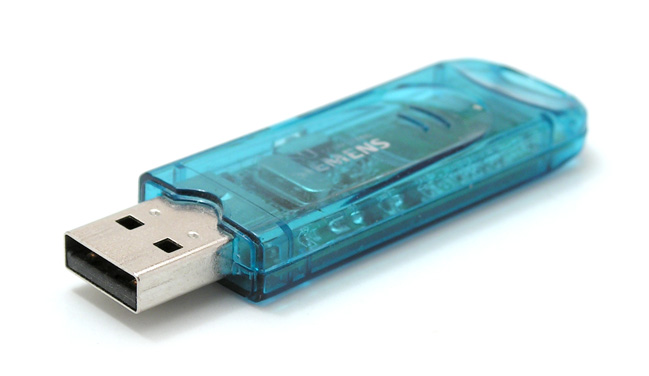
\includegraphics[scale=0.3]{usb_drive.jpg}
		\caption{USB drive}
	\end{figure}		

\newpage
		
		\section{SD Card}
		
	Os \ac{sd} são pequenos cartões que são usados popularmente em câmaras, smartphones e GPS, para fornecer ou aumentar a memória desses dispositivos. Surgiram no ano de 2000 com um armazenamento inicial de 32 \ac{mb}. Existem muitas versões mas a mais conhecida é sem dúvida o micro-SD, o cartão de memória que funciona na maioria dos smartphones.
\vspace{1mm}

	\begin{figure} [h]
		\centering
		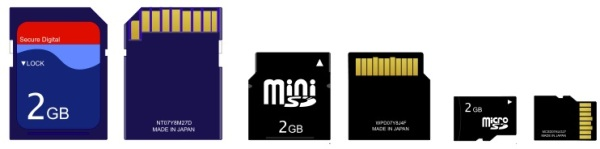
\includegraphics[scale=0.6]{sdcardsizes.jpg}
		\caption{Diferentes tamanhos do Cartão SD}
	\end{figure}
	
	Os cartões de memória \textit{Secure Digital Card}  ou SD Card são uma evolução da tecnologia \textit{MultiMediaCard} (ou MMC). Adicionam capacidades de criptografia e gestão de direitos digitais, adquirindo assim a qualidade de \textit{Secure}, para atender às exigências da indústria da música e um travão para impedir alterações ou a exclusão do conteúdo do cartão.
\vspace{1mm}

	Diferente do que acontece nos discos rígidos, em que o processo de gravação de informações é mecânico, estes cartões utilizam a chamada memória \textit{flash}. Também conhecida como armazenamento sólido, esse tipo de técnica de gravação e leitura acaba por gerar equipamentos mais resistentes a impactos, mais velozes na transferência de dados e com maior durabilidade.
\vspace{1mm}

	Fica na história por ser um dispositivo que não condiciona o tamanho do equipamento onde será usado.
\vspace{1mm}

	\begin{figure} [h]
		\centering
		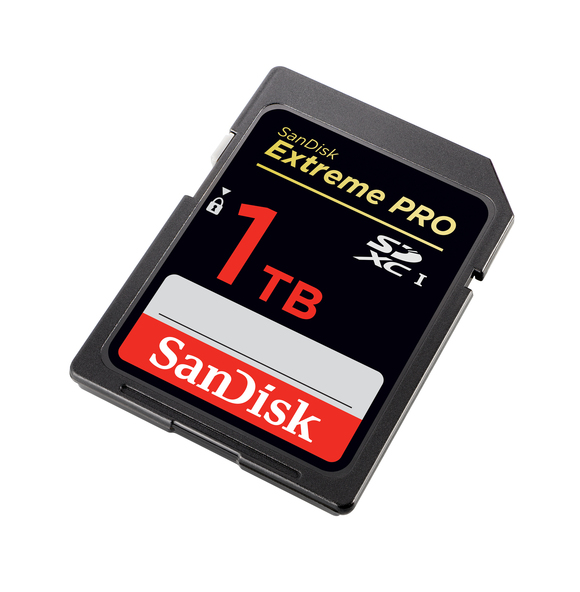
\includegraphics[scale=0.4]{sdcard.jpg}
		\caption{Cartão SD}
	\end{figure}	

\newpage

		\section{Solid-State Drive (SSD)}
		
	O \ac{ssd} é um tipo de dispositivo, sem partes móveis, para armazenamento não volátil de dados digitais. Surgiram em 2008 com um armazenamento inicial de 64 \ac{gb}. São, tipicamente, construídos em torno de um circuito integrado semicondutor, tipicamente memória \textit{NAND Flash}, responsável pelo armazenamento, diferindo dos sistemas magnéticos (como os Discos Rígidos) ou ópticos (discos como CD-Rs). Alguns dos dispositivos mais importantes usam memória \ac{ram} sob condições especiais.
\vspace{5mm}

	\begin{figure} [h]
		\centering
		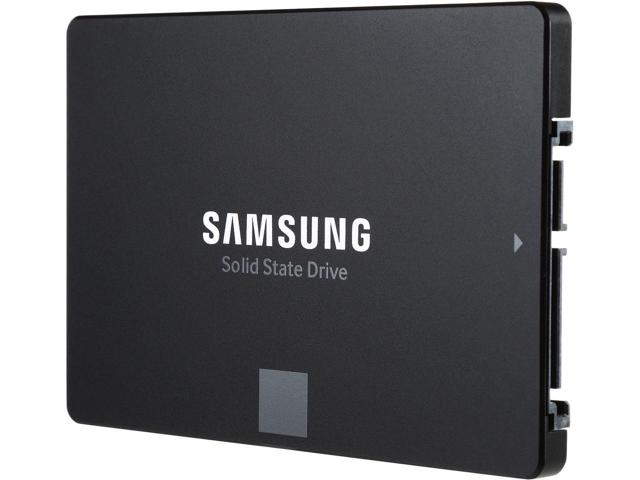
\includegraphics[scale=0.25]{ssd.jpg}
		\caption{Um SSD}
	\end{figure}
	
\vspace{5mm}	
	
	O dispositivo é todo formado por circuitos integrados e em seu interior não há partes móveis, o que o torna absolutamente silencioso, mais rápido e menos propenso a danos físicos do que o disco rígido.
\vspace{1mm}
%referir flash
	O \ac{ssd} possui dois modos de armazenar dados. Temos o sistema de memória \textit{flash}  , método que já foi explicado anteriormente, e a memória \ac{ram} sendo esta menos comum no mundo dos \ac{ssd}. A memória \ac{ram} é um tipo de tecnologia que permite o acesso aos arquivos armazenados no computador. Ao contrário da memória do disco rígido, a \ac{ram} não armazena conteúdos permanentemente. É responsável, no entanto, pela leitura dos conteúdos quando requeridos. Ou seja, de forma não-sequencial. Sendo assim, a memória \ac{ram} pode ser entendida como um espaço temporário de trabalho, pois, após a tarefa estar realizada, os arquivos são retirados da memória e mantidos na unidade principal de memória, neste caso na memória \textit{flash}.
\vspace{1mm}
	
\newpage	
	
	A memória \ac{ram} é um chip semelhante a um micro-processador, composto por milhões de transístores e condensadores. O condensador é uma peça capaz de armazenar eletrões. Quando ele está carregado, o sistema faz uma leitura com base no código binário. Cada leitura dessa em zero ou um significa um bit de informação. Essa leitura é feita de forma muito rápida, são muitas em poucos milésimos de segundos. É assim que a memória \ac{ram} processa todas as ações executadas pelo usuário.
\vspace{20mm}

	\begin{figure} [h]
		\centering
		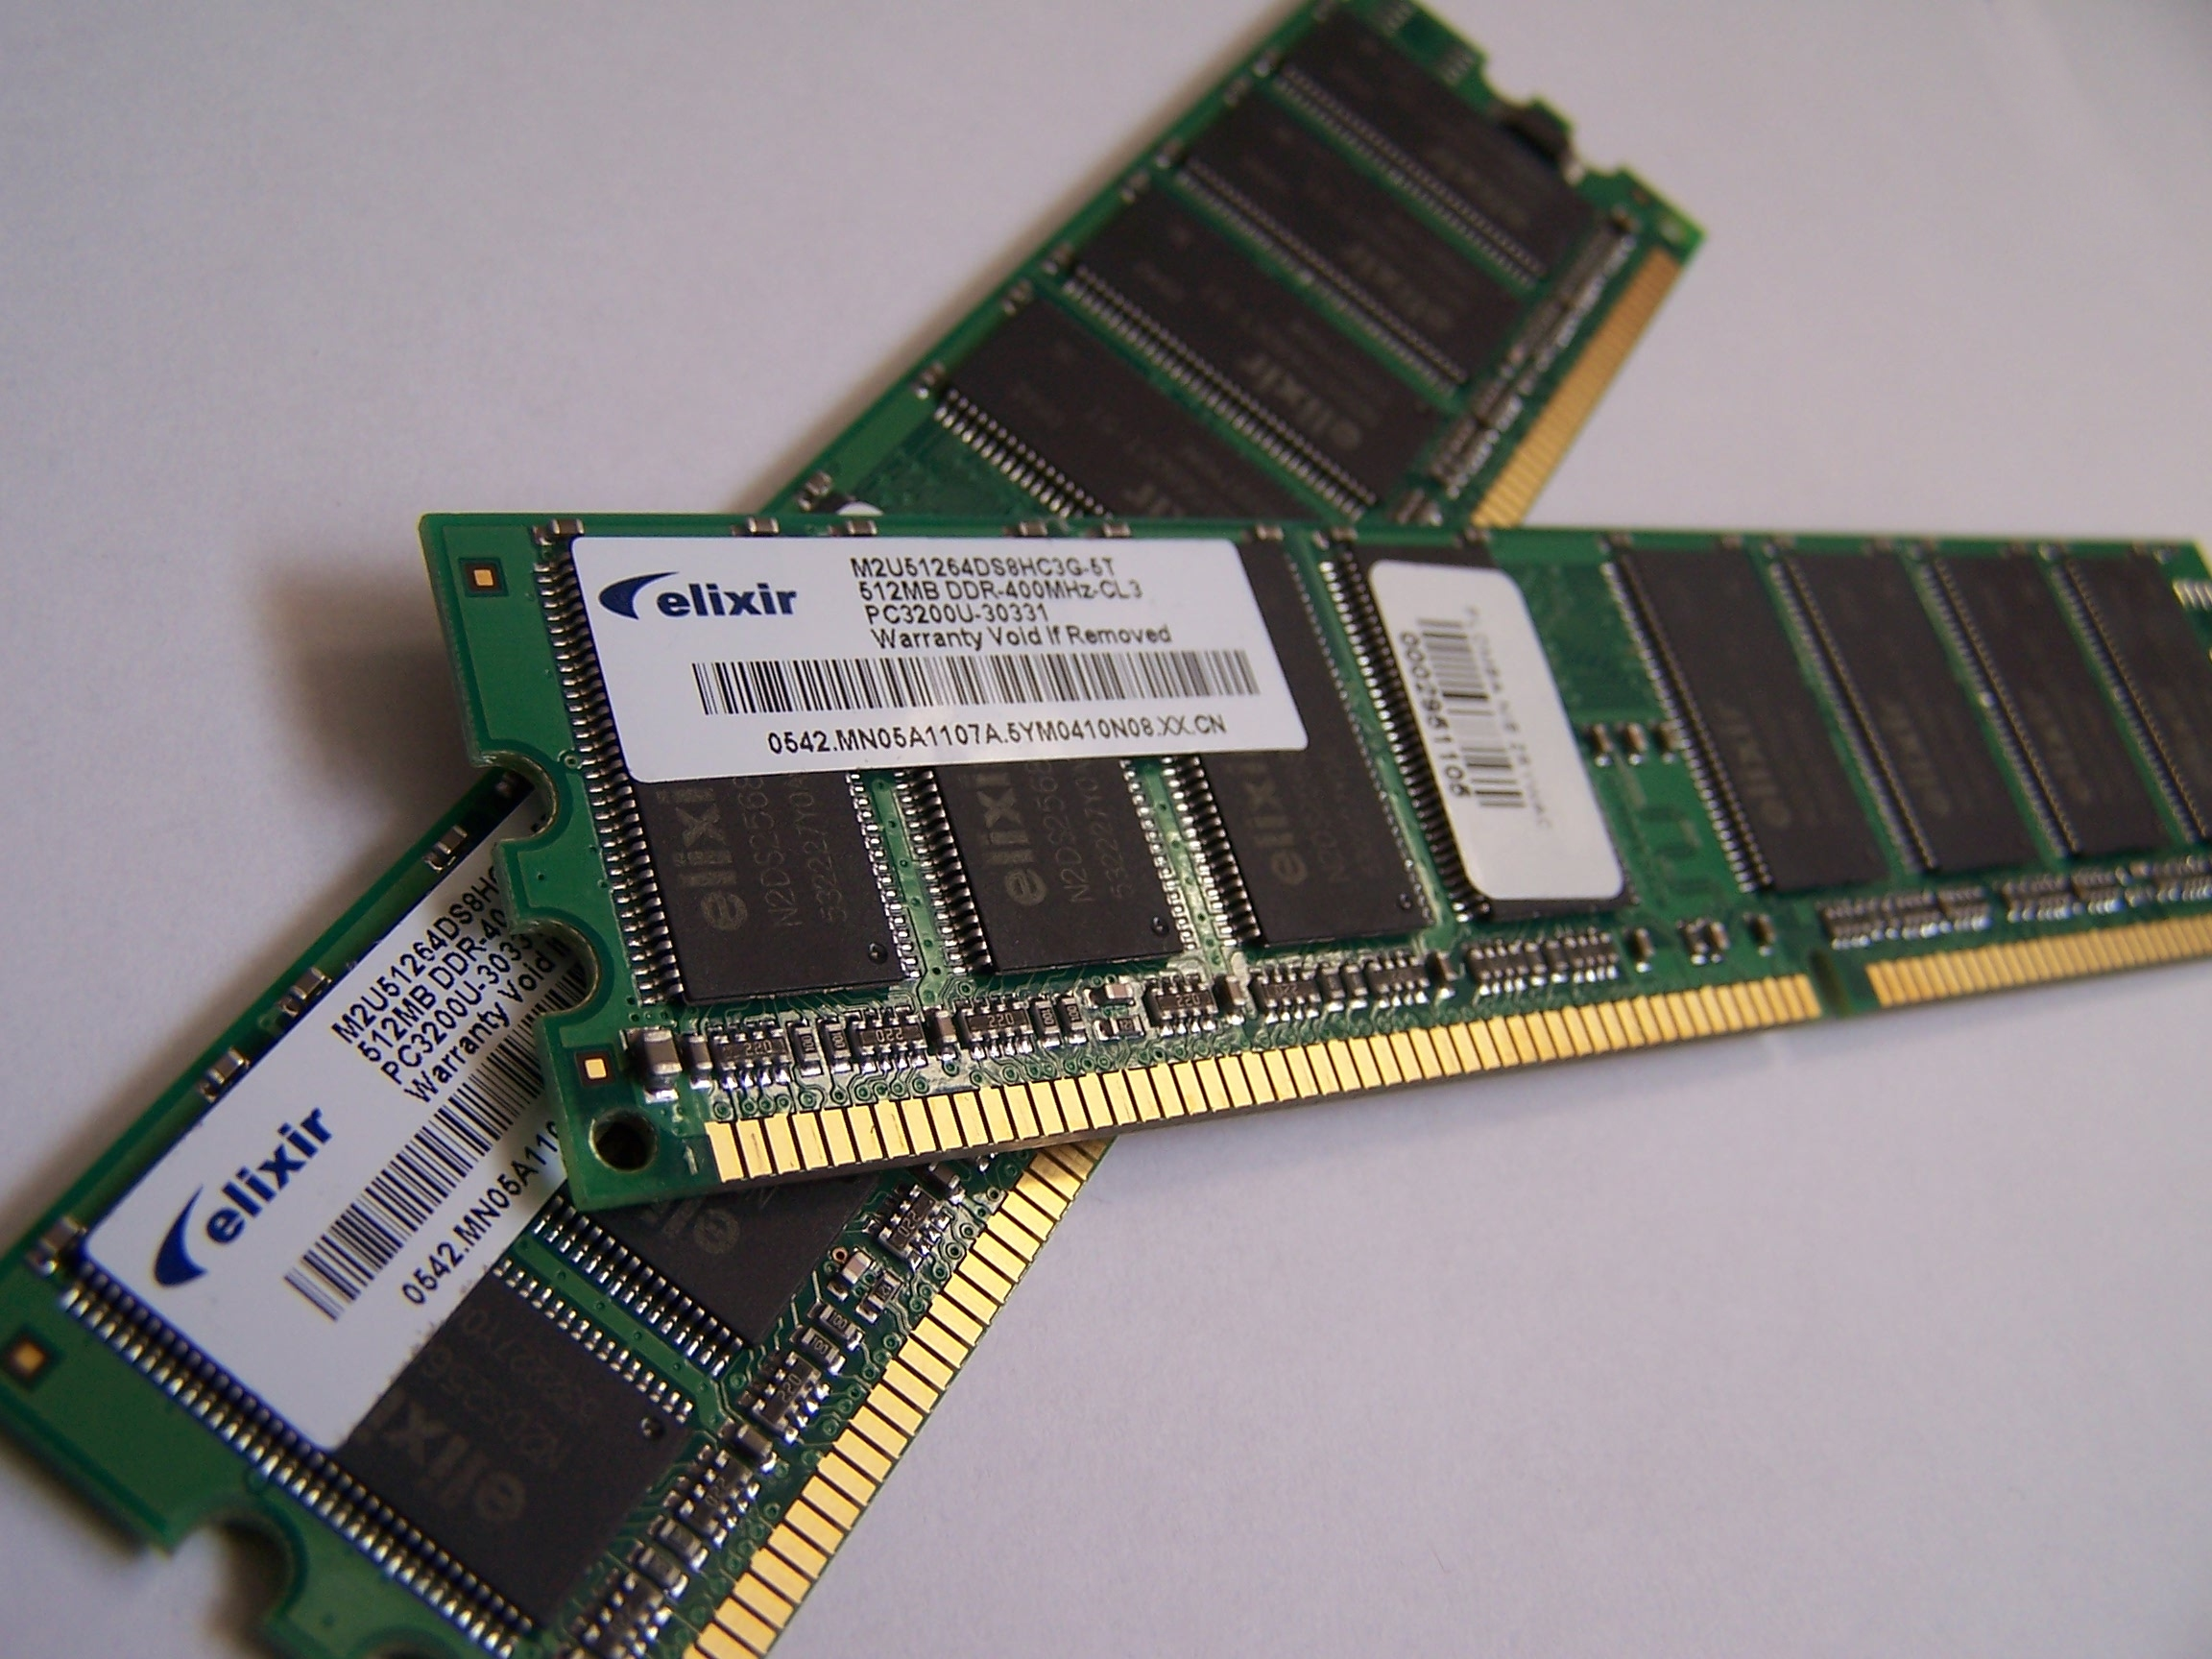
\includegraphics[scale=0.09]{memram.jpg}
		\caption{Memória RAM}
	\end{figure}

\vspace{20mm}	
	
	Assim sendo, o \ac{ssd} deixam a sua marca na história por permitirem tempos de arranque impressionantes e armazenamento seguro. São memórias rápidas e consomem menos energia. São a evolução lógica do alojamento físico. Também podem ser combinadas com discos mecânicos, havendo assim uma unidade híbrida, oferecendo ao consumidor maior oferta.

\newpage

		\section{Cloud Storage}
		
		O \textit{Cloud Storage} é o armazenamento de dados em nuvem, isto é,  os dados são armazenados num local virtual.  Os dados são enviados para servidores remotos e uma vez armazenados, os dados podem ser acessados e compartilhados a partir de qualquer dispositivo conectado à internet.
 Assim, o acesso aos programas, serviços e arquivos é feito remotamente através da internet, a qualquer hora, local, ou mesmo de plataforma. De facto, o único requisito mínimo para utilizar este sistema é mesmo a ligação à internet, não havendo necessidade de instalação de pogramas ou aplicações ou de qualquer outro suporte físico.
\vspace{1mm}

O facto de o \textit{Cloud Storage} permitir o acesso aos dados armazenados remotamente, torna este mesmo sistema mais seguro, pois diminui o risco de perder os dados guardados, podendo mesmo servir de \textit{Backup}. 
Outra vantagem, é ser muito barata e flexível, havendo já serviços grátis com limite de capacidade de armazenamento. 
Uma outra características do Cloud Storage  é a sincronização, que permite que as atualizações de dados sejam compartilhadas em tempo real entre dispositivos. Isto é amplamente explorado por empresas pois permite a trabalhar em equipa.
\vspace{1mm}

	\begin{figure} [b]
		\centering
		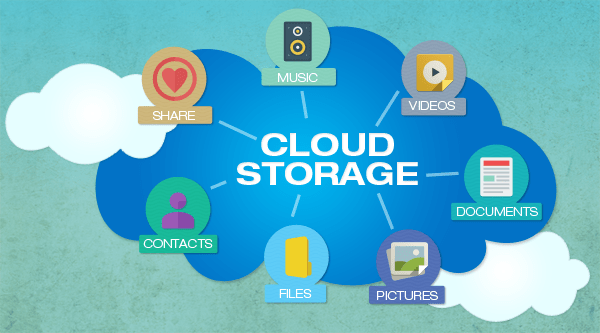
\includegraphics[scale=0.4]{cloud-storage.png}
		\caption{Cloud Storage}
	\end{figure}

A única possível desvantagem do \textit{Cloud Storage} é o acesso aos dados ser feito exclusivamente pela internet. Em alguns casos, a ligação à internet pode ser impossível ou fraca e o acesso aos dados é negado.

\newpage

Todas estas características fazem com que o \textit{Cloud Storage} tenha vindo a ganhar cada vez mais adesão, sendo já usada por milhões de utilizadores, seja por motivos laborais ou pessoais.
\vspace{1mm}

	Alguns exemplos de Cloud Storage são:
	\begin{enumerate}
		\item CloudPT
		\item  Dropbox
		\item  IDrive
		\item Sugarsync
		\item Memopal
		\item Mozy
		\item ADrive
		\item Duplicati
		\item Box
		\item CloudMe
	\end{enumerate} 
	
\vspace{15mm}
 
 	\begin{figure} [h]
		\centering
		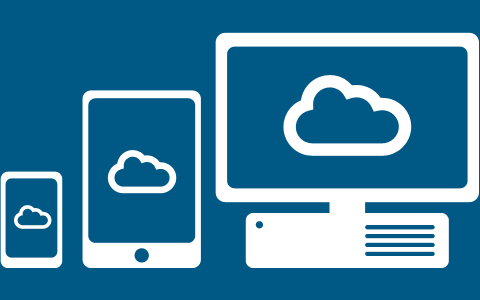
\includegraphics[scale=0.5]{cloud-storage2.png}
		\caption{Alguns dispositivos que podem usar Cloud Storage}
	\end{figure}
	
%\chapter{Análise}
%\label{chap.analise}
%Analisa os resultados.

\chapter{Conclusões Finais}
\label{chap.conclusao}

	Os dispositivos de armazenamento de dados são necessários para o nosso dia a dia cada vez mais, seja a nível profissional ou para fins de lazer. Sendo o seu uso tão necessário, é trivial que estes tendam a evoluir em todos os aspetos possíveis, seja a nível dimensional, velocidade de acesso e nos seus métodos de gravação. Sendo assim, e com os olhos colocados no futuro, é esperado uma otimização nestes sistemas levada ao extremo, com dispositivos que cabem na palma da nossa mão, moveis e com maior capacidade de armazenamento que os dispositivos do nosso presente.

 
\chapter*{Contribuições dos autores}
completar amanha

Afonso Cardoso - 50 \%
Pedro Almeida -50 \%

%%%%%%%%%%%%%%%%%%%%%%%%%%%%%%%%%
\chapter*{Acrónimos}
\begin{acronym}
\acro{ua}[UA]{Universidade de Aveiro}
\acro{miect}[MIECT]{Mestrado Integrado em Engenharia de Computadores e Telemática}
\acro{lei}[LEI]{Licenciatura em Engenharia Informática}
\acro{glisc}[GLISC]{Grey Literature International Steering Committee}
\acro{ibm}[IBM]{International Business Machines}
\acro{ramac}[RAMAC]{Random Access Method of Accounting and Control}
\acro{kb}[KB]{Kilobyte}
\acro{mb}[MB]{Megabyte}
\acro{gb}[GB]{Gigabyte}
\acro{ssd}[SSD]{Solid-State Drive}
\acro{ram}[RAM]{Random Acess Memory}
\acro{mmc}[MMC]{MultiMediaCard}
\acro{fdd}[FDD]{Floppy Disk Drive}
\acro{dasd}[DASD]{Direct Access Storage Device}
\acro{mfm}[MFM]{Modified Frequency Modulation}
\acro{dat}[DAT]{Digital Audio Tape}
\acro{md}[MD]{MiniDisc Data}
\acro{sd}[SD]{Secure Digital Card}
\end{acronym}


%%%%%%%%%%%%%%%%%%%%%%%%%%%%%%%%%
\printbibliography

\end{document}
